\documentclass[11pt]{article}

% ---------- Basic packages ----------
\usepackage[T1]{fontenc}
\usepackage{lmodern}
\usepackage{microtype}
\usepackage[margin=1in,headheight=15pt]{geometry}
\usepackage{graphicx}
\usepackage{amsmath,amssymb,amsthm}
\usepackage{mathtools}
\usepackage{tikz}
\usetikzlibrary{arrows.meta}
\usepackage{pgfplots}
\usepgfplotslibrary{groupplots}
\pgfplotsset{compat=1.18}
\usepackage[most]{tcolorbox}
\usepackage{xcolor}
\usepackage{fancyhdr}
\usepackage{titlesec}
\usepackage{enumitem}
\usepackage[hidelinks]{hyperref}
\usepackage{cleveref}
\usepackage{float}
\setlength{\parindent}{0pt}
\setlength{\parskip}{6pt}

% ---------- Document information ----------
\author{Ellie Su}
\hypersetup{
    pdftitle={Fourier Series: From Orthogonal Vectors to Heat Flow},
    pdfauthor={Ellie Su and Dawon Suh}
}

% ---------- Colors ----------
\definecolor{deepblue}{HTML}{315A78}
\definecolor{softblue}{HTML}{EFF7FC}

\definecolor{purple}{HTML}{745A8D}
\definecolor{softpurple}{HTML}{F5F0FA}

\definecolor{green}{HTML}{527A63}
\definecolor{softgreen}{HTML}{EFF8F3}

\definecolor{pink}{HTML}{A76578}
\definecolor{softpink}{HTML}{FFF2F5}

\definecolor{gold}{HTML}{A78032}
\definecolor{softyellow}{HTML}{FFF9E8}

\definecolor{softgray}{HTML}{F7F7F7}
\definecolor{grayborder}{HTML}{888888}

% ---------- Theorem environments ----------
\newtheorem{theorem}{Theorem}[section]
\newtheorem{lemma}[theorem]{Lemma}
\newtheorem{proposition}[theorem]{Proposition}
\newtheorem{corollary}[theorem]{Corollary}

\theoremstyle{definition}
\newtheorem{definition}[theorem]{Definition}
\newtheorem{example}[theorem]{Example}
\newtheorem{problem}[theorem]{Problem}
\newtheorem{salvage}[theorem]{Salvage}

\theoremstyle{remark}
\newtheorem{remark}[theorem]{Remark}

% ---------- Proof-style environments ----------
\newenvironment{disproof}
    {\begin{proof}[Disproof]}
    {\end{proof}}

\newenvironment{solution}
    {\begin{proof}[Solution]}
    {\end{proof}}

% ---------- General box style ----------
\tcbset{
    mathematicalbox/.style={
        enhanced,
        breakable,
        boxrule=0.8pt,
        arc=2.5mm,
        left=10pt,
        right=10pt,
        top=8pt,
        bottom=8pt,
        before skip=10pt,
        after skip=10pt,
        fonttitle=\bfseries
    }
}

% ---------- General-purpose box ----------
\newtcolorbox{mathbox}[1][]{
    mathematicalbox,
    colback=white,
    colframe=deepblue,
    coltitle=deepblue,
    borderline west={3pt}{0pt}{deepblue},
    #1
}

% ---------- Theorem and proposition boxes ----------
\tcolorboxenvironment{theorem}{
    mathematicalbox,
    colback=softblue,
    colframe=deepblue,
    borderline west={3pt}{0pt}{deepblue}
}

\tcolorboxenvironment{proposition}{
    mathematicalbox,
    colback=softblue,
    colframe=deepblue,
    borderline west={3pt}{0pt}{deepblue}
}

% ---------- Lemma boxes ----------
\tcolorboxenvironment{lemma}{
    mathematicalbox,
    colback=softpurple,
    colframe=purple,
    borderline west={3pt}{0pt}{purple}
}

% ---------- Corollary boxes ----------
\tcolorboxenvironment{corollary}{
    mathematicalbox,
    colback=softgreen,
    colframe=green,
    borderline west={3pt}{0pt}{green}
}

% ---------- Definition boxes ----------
\tcolorboxenvironment{definition}{
    mathematicalbox,
    colback=softpink,
    colframe=pink,
    borderline west={3pt}{0pt}{pink}
}

% ---------- Example boxes ----------
\tcolorboxenvironment{example}{
    mathematicalbox,
    colback=softgreen,
    colframe=green,
    borderline west={3pt}{0pt}{green}
}

% ---------- Problem boxes ----------
\tcolorboxenvironment{problem}{
    mathematicalbox,
    colback=softyellow,
    colframe=gold,
    borderline west={3pt}{0pt}{gold}
}

% ---------- Salvage boxes ----------
\tcolorboxenvironment{salvage}{
    mathematicalbox,
    colback=softpurple,
    colframe=purple,
    borderline west={3pt}{0pt}{purple}
}

% ---------- Remark boxes ----------
\tcolorboxenvironment{remark}{
    enhanced,
    breakable,
    colback=white,
    colframe=grayborder,
    boxrule=0.7pt,
    arc=2.5mm,
    left=10pt,
    right=10pt,
    top=8pt,
    bottom=8pt,
    before skip=10pt,
    after skip=10pt,
    frame style={
        dash pattern=on 3pt off 2pt
    }
}

% ---------- Proof, disproof, and solution boxes ----------
\tcolorboxenvironment{proof}{
    enhanced,
    breakable,
    colback=softgray,
    colframe=grayborder,
    boxrule=0.5pt,
    arc=2mm,
    left=10pt,
    right=10pt,
    top=8pt,
    bottom=8pt,
    before skip=8pt,
    after skip=10pt,
    borderline west={2pt}{0pt}{grayborder}
}

% ---------- Section headings ----------
\titleformat{\section}
    {\Large\bfseries\color{deepblue}}
    {\thesection.}
    {0.5em}
    {}
    [\vspace{2pt}\color{deepblue}\titlerule]

\titleformat{name=\section,numberless}
    {\Large\bfseries\color{deepblue}}
    {}
    {0pt}
    {}
    [\vspace{2pt}\color{deepblue}\titlerule]

\titleformat{\subsection}
    {\large\bfseries\color{purple}}
    {\thesubsection.}
    {0.5em}
    {}

\titleformat{name=\subsection,numberless}
    {\large\bfseries\color{purple}}
    {}
    {0pt}
    {}

\titlespacing*{\section}
    {0pt}
    {18pt}
    {8pt}

\titlespacing*{\subsection}
    {0pt}
    {14pt}
    {5pt}

% ---------- Lists ----------
\setlist[enumerate]{
    itemsep=3pt,
    topsep=5pt,
    leftmargin=*
}

\setlist[itemize]{
    itemsep=3pt,
    topsep=5pt,
    leftmargin=*
}

% ---------- Header and footer ----------
\pagestyle{fancy}
\fancyhf{}

\fancyhead[L]{
    \small\textcolor{deepblue}{HRK notes}
}

\fancyhead[R]{
    \small\textcolor{deepblue}{Ellie Su}
}

\fancyfoot[C]{
    \small\textcolor{grayborder}{\thepage}
}

\renewcommand{\headrulewidth}{0.4pt}
\renewcommand{\footrulewidth}{0pt}

% ---------- Custom title ----------
\newcommand{\settitle}[2]{%
    \thispagestyle{fancy}

    \begingroup
    \centering

    \vspace*{-0.65cm}

    {\color{deepblue}
    \rule{0.72\textwidth}{1.1pt}\par}

    \vspace{0.35cm}

    {\fontsize{30}{34}\selectfont
    \bfseries
    \color{deepblue}
    #1\par}

    \vspace{0.2cm}

    {\small
    \color{grayborder}
    #2\par}

    \vspace{0.35cm}

    {\color{deepblue}
    \rule{0.72\textwidth}{0.7pt}\par}

    \vspace{0.5cm}

    \endgroup
}

% ---------- Notation ----------
\numberwithin{equation}{section}
\newcommand{\CC}{\mathbb{C}}
\newcommand{\ZZ}{\mathbb{Z}}
\newcommand{\RR}{\mathbb{R}}
\newcommand{\ee}{\mathrm{e}}
\newcommand{\norm}[1]{\left\lVert#1\right\rVert}
\newcommand{\ip}[2]{\left\langle#1,#2\right\rangle}
\newcommand{\mean}[1]{\overline{#1}}
\DeclareMathOperator{\sgn}{sgn}

% ---------- Document ----------
\begin{document}

\settitle{Fourier Series}{From Orthogonal Vectors to Heat Flow\\[3pt]
Ellie Su and Dawon Suh \quad | \quad July 2026}

% Fourier Series chapter content for main.tex
% All theorem, example, definition, and proof styles are defined in main.tex.

\section{Motivation: complicated shapes from simple waves}
A sine wave is smooth and regular. Yet sums of sine waves can approximate sharp
corners and even jumps. The plots below show three periodic patterns that we will
study in this article.

\begin{figure}[htbp]
\centering
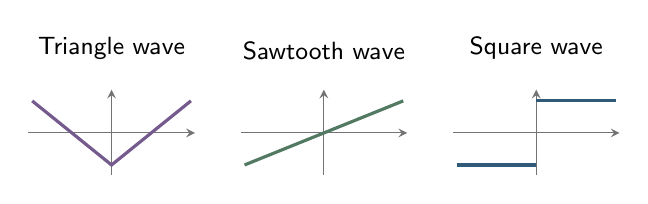
\begin{tikzpicture}
\begin{groupplot}[
 group style={group size=3 by 1,horizontal sep=0.58cm},
 width=0.305\textwidth,height=0.22\textwidth,
 axis lines=middle, xmin=-3.3,xmax=3.3,ymin=-1.32,ymax=1.35,
 xtick=\empty,ytick=\empty,
 axis line style={black!55},
 title style={font=\small\sffamily,at={(0.5,1.05)},anchor=south},
 every axis plot/.append style={line width=1.15pt},
 clip=false]
\nextgroupplot[title={Triangle wave}]
\addplot[color=purple] coordinates {(-3.14159,1) (0,-1) (3.14159,1)};
\nextgroupplot[title={Sawtooth wave}]
\addplot[color=green] coordinates {(-3.14159,-1) (3.14159,1)};
\nextgroupplot[title={Square wave}]
\addplot[color=deepblue] coordinates {(-3.14159,-1) (0,-1)};
\addplot[color=deepblue] coordinates {(0,1) (3.14159,1)};
\end{groupplot}
\end{tikzpicture}
\caption{One period of three functions, continued periodically beyond the window.
The vertical jump in the square wave is intentionally left disconnected.}
\label{fig:three-waves}
\end{figure}

The guiding question is:
\begin{center}
\emph{Can we express a complicated periodic function as a linear combination of simple oscillations?}
\end{center}

For a function of period $2\pi$, the complex Fourier series has the form
\begin{equation}\label{eq:fourier-proposal}
 f(x)\sim\sum_{n=-\infty}^{\infty}c_n\ee^{inx}.
\end{equation}
Here $n\in\ZZ$ labels the \emph{frequency}, while $c_n\in\CC$ records the
strength and phase of that frequency. By Euler's formula,
\[
 \ee^{inx}=\cos(nx)+i\sin(nx),
\]
so the complex exponential conveniently packages both sine and cosine waves.
We use the symbol $\sim$ for now: the question of when the series actually equals
$f$ requires a separate convergence theorem (\cref{sec:convergence}).

\section{Preliminaries: treating functions as vectors}
\subsection{Inner products in finite dimensions}
\begin{definition}[Complex inner product]
For vectors $v=(v_1,\dots,v_m)$ and $w=(w_1,\dots,w_m)$ in $\CC^m$, define
\begin{equation}\label{eq:vector-ip}
 \ip{v}{w}=\sum_{j=1}^m v_j\overline{w_j}.
\end{equation}
We use the convention that the inner product is \emph{linear in its first entry}
and conjugate-linear in its second. Two vectors are \emph{orthogonal} if their
inner product is zero; they are \emph{orthonormal} if they are orthogonal
and each has norm $1$.
\end{definition}
The complex conjugate is essential because
\[
 \ip{v}{v}=\sum_{j=1}^m |v_j|^2\geq0,
 \qquad \norm{v}=\sqrt{\ip{v}{v}}.
\]
Without conjugation, the ``squared length'' could be negative or nonreal.

\begin{proposition}[Extracting coefficients by projection]\label{prop:projection}
If $e_1,\ldots,e_m$ are nonzero, mutually orthogonal vectors and
$v=\sum_{j=1}^m c_je_j$, then
\begin{equation}\label{eq:projection}
 \boxed{c_k=\frac{\ip{v}{e_k}}{\ip{e_k}{e_k}}.}
\end{equation}
For an orthonormal basis, the denominator is $1$.
\end{proposition}
\begin{proof}
By linearity and orthogonality,
\[
 \ip{v}{e_k}=\sum_{j=1}^m c_j\ip{e_j}{e_k}
 =c_k\ip{e_k}{e_k}.
\]
Dividing by the nonzero squared norm gives the result.
\end{proof}

\subsection{Inner products for functions}
\begin{definition}[The $L^2$ inner product]\label{def:L2}
For square-integrable complex-valued functions on $[-\pi,\pi]$, define
\begin{equation}\label{eq:function-ip}
 \ip{f}{g}=\int_{-\pi}^{\pi}f(x)\overline{g(x)}\,dx,
 \qquad
 \norm{f}=\left(\int_{-\pi}^{\pi}|f(x)|^2\,dx\right)^{1/2}.
\end{equation}
The space $L^2[-\pi,\pi]$ consists of square-integrable functions, with functions
identified when they agree almost everywhere.
\end{definition}
The integral replaces the finite sum in the vector inner product. We can
therefore study a function using coordinates along an orthogonal family of functions.
The qualifier ``almost everywhere'' matters: changing the value of a function
at finitely many points does not change any of its Fourier coefficients.

\begin{remark}
\textbf{The central analogy.} In ordinary Euclidean space, choosing orthogonal
coordinate axes makes a vector easy to describe. In a function space, choosing
orthogonal oscillations makes a function easy to describe. Fourier coefficients
are the coordinates of a function along those oscillatory directions.
\end{remark}

\section{Deriving the complex Fourier coefficients}
\subsection{Orthogonality of complex exponentials}
For each integer $n$, define the Fourier mode $e_n(x)=\ee^{inx}$.

\begin{lemma}[Orthogonality of Fourier modes]\label{lem:orthogonality}
For all integers $n$ and $m$,
\begin{equation}\label{eq:orthogonality}
 \boxed{\ip{e_n}{e_m}=\begin{cases}
 2\pi,&n=m,\\[2pt]0,&n\neq m.
 \end{cases}}
\end{equation}
Thus the normalized functions $\phi_n(x)=\ee^{inx}/\sqrt{2\pi}$
form an orthonormal family in $L^2[-\pi,\pi]$.
\end{lemma}
\begin{proof}
Using the definition of the complex inner product,
\begin{align*}
 \ip{e_n}{e_m}
 &=\int_{-\pi}^{\pi}\ee^{inx}\overline{\ee^{imx}}\,dx\\
 &=\int_{-\pi}^{\pi}\ee^{i(n-m)x}\,dx.
\end{align*}
If $n\neq m$, the integral equals
\[
 \left.\frac{\ee^{i(n-m)x}}{i(n-m)}\right|_{-\pi}^{\pi}
 =\frac{\ee^{i(n-m)\pi}-\ee^{-i(n-m)\pi}}{i(n-m)}=0,
\]
because both exponentials in the numerator equal $(-1)^{n-m}$.
If $n=m$, the integrand is $1$ and the integral is $2\pi$.
Hence $\norm{e_n}=\sqrt{2\pi}$, giving the stated normalization.
\end{proof}

\subsection{Projecting onto a Fourier mode}
First suppose $f$ is a \emph{finite} trigonometric sum,
$f(x)=\sum_{n=-N}^{N}c_ne_n(x)$. Taking the inner product with $e_m$ gives
\[
 \ip{f}{e_m}
 =\sum_{n=-N}^{N}c_n\ip{e_n}{e_m}
 =2\pi c_m \qquad (|m|\leq N).
\]
This is the same projection principle as in \cref{prop:projection}.
The calculation motivates the general coefficient formula.

\begin{definition}[Complex Fourier coefficients]\label{def:fourier-coeff}
For $f\in L^2[-\pi,\pi]$, its $n$th complex Fourier coefficient is
\begin{equation}\label{eq:coefficients}
 \boxed{c_n=\frac{1}{2\pi}\int_{-\pi}^{\pi}f(x)\ee^{-inx}\,dx,
 \qquad n\in\ZZ.}
\end{equation}
The corresponding formal Fourier series is
\begin{equation}\label{eq:series}
 \boxed{f(x)\sim\sum_{n\in\ZZ}c_n\ee^{inx}.}
\end{equation}
The symbol $\sim$ reminds us that the meaning of reconstruction
must be addressed separately.
\end{definition}

\begin{theorem}[Completeness of the complex exponentials]\label{thm:completeness}
The functions $\{\ee^{inx}/\sqrt{2\pi}:n\in\ZZ\}$ form a complete
orthonormal basis of $L^2[-\pi,\pi]$. Consequently, the symmetric
Fourier partial sums
\[
 S_Nf(x)=\sum_{n=-N}^{N}c_n\ee^{inx}
\]
converge to $f$ in the $L^2$ norm as $N\to\infty$.
\end{theorem}
The completeness assertion is a separate, nontrivial result.
The orthogonality calculation identifies \emph{which} coefficients an
expansion must have; completeness explains \emph{why} those coefficients
recover an arbitrary $L^2$ function in mean square. We state this theorem
without proving its full functional-analytic content.

\section{The real Fourier series and symmetry}
Many physical functions are real-valued. Pairing positive and negative
frequencies in \cref{eq:series} gives an equivalent sine-and-cosine expansion.

\begin{proposition}[Real Fourier coefficients]\label{prop:real}
For a real-valued $2\pi$-periodic function $f\in L^2[-\pi,\pi]$,
\begin{equation}\label{eq:real-series}
 f(x)\sim\frac{a_0}{2}
 +\sum_{n=1}^{\infty}\bigl(a_n\cos(nx)+b_n\sin(nx)\bigr),
\end{equation}
where
\begin{align}\label{eq:real-coeffs}
 a_n&=\frac{1}{\pi}\int_{-\pi}^{\pi}f(x)\cos(nx)\,dx
 &&(n\geq0),\\
 b_n&=\frac{1}{\pi}\int_{-\pi}^{\pi}f(x)\sin(nx)\,dx
 &&(n\geq1).
\end{align}
In complex notation,
\[
 c_0=\frac{a_0}{2},\qquad
 c_n=\frac{a_n-ib_n}{2},\qquad
 c_{-n}=\frac{a_n+ib_n}{2} \quad (n\geq1).
\]
\end{proposition}
\begin{proof}
For real $f$, conjugating the coefficient integral shows
$c_{-n}=\overline{c_n}$. Now group the $n$ and $-n$ terms:
\[
 c_n\ee^{inx}+c_{-n}\ee^{-inx}
 =(c_n+c_{-n})\cos(nx)+i(c_n-c_{-n})\sin(nx).
\]
Substituting the coefficient integrals yields the stated formulas.
\end{proof}

Symmetry often saves half the integration:
\begin{itemize}
 \item If $f(-x)=f(x)$ (\emph{even}), then $b_n=0$ and only cosines appear.
 \item If $f(-x)=-f(x)$ (\emph{odd}), then $a_n=0$ and only sines appear.
\end{itemize}
The constant coefficient has a particularly useful interpretation:
\begin{equation}\label{eq:mean}
 c_0=\frac{1}{2\pi}\int_{-\pi}^{\pi} f(x)\,dx
 =\text{the average value of }f\text{ over one period}.
\end{equation}

\section{Three worked examples}\label{sec:examples}
These calculations show why the elementary wave shapes in
\cref{fig:three-waves} can be built from trigonometric functions.

\begin{example}[Sawtooth wave: $f(x)=x$]
Let $f(x)=x$ for $-\pi<x<\pi$, extended $2\pi$-periodically. Since $f$ is odd,
only sine terms survive. Integration by parts gives
\begin{align*}
 b_n&=\frac{1}{\pi}\int_{-\pi}^{\pi}x\sin(nx)\,dx
 =\frac{2}{\pi}\int_0^\pi x\sin(nx)\,dx\\
 &=\frac{2}{\pi}\left[-\frac{x\cos(nx)}n+\frac{\sin(nx)}{n^2}\right]_0^\pi
 =\frac{2(-1)^{n+1}}n.
\end{align*}
Therefore,
\begin{equation}\label{eq:sawtooth}
 \boxed{x\sim 2\sum_{n=1}^{\infty}\frac{(-1)^{n+1}}n\sin(nx),
 \qquad -\pi<x<\pi.}
\end{equation}
At the periodic jump $x=\pi$ (equivalently $x=-\pi$), the series converges
to $0$, the average of the one-sided limits $\pi$ and $-\pi$.

\end{example}

\begin{example}[Square wave: only odd harmonics]
Define the periodic square wave by
\[
 f(x)=\begin{cases}
 -1,&-\pi<x<0,\\
 1,&0<x<\pi.
 \end{cases}
\]
The values at the jump points can be chosen separately. Again $f$ is odd,
so $a_n=0$. We find
\[
 b_n=\frac{2}{\pi}\int_0^\pi\sin(nx)\,dx
 =\frac{2}{\pi n}\bigl(1-(-1)^n\bigr)
 =\begin{cases}4/(\pi n),&n\text{ odd},\\0,&n\text{ even}.
 \end{cases}
\]
Consequently,
\begin{equation}\label{eq:square}
 \boxed{f(x)\sim\frac{4}{\pi}\left(
 \sin x+\frac{\sin3x}{3}+\frac{\sin5x}{5}+\cdots\right).}
\end{equation}
Near a jump, the partial sums oscillate and overshoot. This behavior is
called the \emph{Gibbs phenomenon}, discussed further in
\cref{sec:convergence}.

\end{example}

\begin{example}[Triangle wave: $f(x)=|x|$]
Let $f(x)=|x|$ on $[-\pi,\pi]$ and extend periodically. This function is even,
so it has only cosines. Its average is $a_0/2=\pi/2$, while
\begin{align*}
 a_n&=\frac{2}{\pi}\int_0^\pi x\cos(nx)\,dx\\
 &=\frac{2}{\pi}\left[
 \frac{x\sin(nx)}n+\frac{\cos(nx)}{n^2}\right]_0^\pi
 =\frac{2}{\pi}\frac{(-1)^n-1}{n^2}.
\end{align*}
Thus $a_n=0$ for even $n$, and $a_n=-4/(\pi n^2)$ for odd $n$:
\begin{equation}\label{eq:triangle}
 \boxed{|x|=\frac{\pi}{2}-\frac4\pi\left(
 \cos x+\frac{\cos3x}{3^2}+\frac{\cos5x}{5^2}+\cdots\right).}
\end{equation}
Unlike the sawtooth and square-wave series, the coefficients here decay like
$1/n^2$, so their absolute sum is finite. The triangle wave is continuous,
although its corners make it nondifferentiable at certain points.
\end{example}

\begin{remark}
\textbf{Smoothness versus frequency.} Abrupt jumps require a relatively large
contribution from high frequencies. Smoother functions tend to have smaller
high-frequency coefficients. For example, periodic integration by parts gives
$c_n=(in)^{-1}\widehat{f'}_n$ when $f$ is sufficiently smooth and periodic;
each additional justified integration by parts introduces another factor $1/n$.
\end{remark}

\section{What does convergence mean?}\label{sec:convergence}
For $N\geq0$, the \emph{symmetric partial sum} is
\[
 S_Nf(x)=\sum_{n=-N}^{N}c_n\ee^{inx}.
\]
A Fourier series need not recover the prescribed value of its function at
every point. Two kinds of convergence are especially important.

\begin{theorem}[Pointwise convergence under Dirichlet conditions]\label{thm:dirichlet}
If a periodic function is piecewise continuously differentiable on a period,
with only finitely many discontinuities and finite one-sided limits, then
\begin{equation}\label{eq:dirichlet}
 \lim_{N\to\infty} S_Nf(x)=\frac{f(x^-)+f(x^+)}{2}.
\end{equation}
At a point of continuity, this is $f(x)$; at a jump, it is the midpoint
of the left and right limits.
\end{theorem}
The hypothesis is sufficient rather than necessary. In particular, it
explains why the sawtooth and square-wave Fourier series converge to the
midpoint at a jump, even if the original function is defined differently there.

\begin{theorem}[Mean-square convergence and Parseval's identity]
For every $f\in L^2[-\pi,\pi]$,
\begin{equation}\label{eq:l2-convergence}
 \lim_{N\to\infty}\int_{-\pi}^{\pi}|f(x)-S_Nf(x)|^2\,dx=0.
\end{equation}
Moreover, its Fourier coefficients satisfy
\begin{equation}\label{eq:parseval}
 \boxed{\frac1{2\pi}\int_{-\pi}^{\pi}|f(x)|^2\,dx
 =\sum_{n\in\ZZ}|c_n|^2.}
\end{equation}
\end{theorem}
The first conclusion means that the \emph{integrated squared error}
tends to zero; it does not by itself claim convergence at each point.
Parseval's identity equates the total squared size of a function with the sum
of the squared magnitudes of its Fourier coefficients.

\begin{remark}
\textbf{Gibbs phenomenon.} Near a jump, Fourier partial sums may overshoot.
For a standard jump discontinuity, the limiting overshoot on each side is
approximately $8.95\%$ of the jump height. Adding more terms makes the
oscillating region narrower, but does not remove this limiting overshoot.
\end{remark}

\section{Historical interlude}
In 1807, Joseph Fourier submitted a memoir on heat conduction to the Paris
Academy of Sciences. One of his central claims was that highly general
functions could be represented by trigonometric series. This was controversial:
finite sums of sines and cosines are smooth, so how could an infinite sum
possibly represent a function with a corner or jump?

Fourier developed his methods in \emph{Th\'eorie analytique de la chaleur}
(1822), but the precise meaning and validity of such expansions still required
careful mathematical analysis. Subsequent work, including that of Dirichlet,
helped clarify sufficient conditions for convergence. These questions also
contributed to the development of rigorous notions of functions, integration,
and limits. The history teaches an important lesson: a powerful calculation can
come before a complete account of why it works.

\section{Application: solving the heat equation}\label{sec:heat}
\subsection{Physical setup and boundary conditions}
Consider a thin circular metal rod, or a wire bent into a ring, with
circumference $2\pi$. Assume that heat flows along the ring, the material is
uniform, and no heat escapes to the surroundings. Let $u(x,t)$ denote its
temperature at location $x$ and time $t$, with thermal diffusivity $\kappa>0$.
Fourier's law of heat conduction says that the heat flux along the ring is
$q=-K u_x$, where $K$ is the thermal conductivity. Conservation of thermal
energy gives $\rho c_p u_t=-q_x=K u_{xx}$, where $\rho$ is density and
$c_p$ is specific heat capacity. Hence $\kappa=K/(\rho c_p)$ and the
heat equation and periodic boundary conditions are
\begin{equation}\label{eq:heat-pde}
 \begin{cases}
 u_t=\kappa u_{xx}, &-\pi<x<\pi,\quad t>0,\\
 u(-\pi,t)=u(\pi,t),&t>0,\\
 u_x(-\pi,t)=u_x(\pi,t),&t>0,\\
 u(x,0)=f(x),&-\pi<x<\pi.
 \end{cases}
\end{equation}

The second derivative measures the local curvature of the temperature profile.
Where a point is colder than its nearby surroundings, this curvature is often
positive and the point warms; where it is hotter, the curvature is often
negative and the point cools. Thus \emph{temperature does not necessarily
decrease at each location}. Instead, nonuniformities disappear over time.

\subsection{A single frequency evolves independently}
The key identity is
\begin{equation}\label{eq:eigen}
 \frac{d^2}{dx^2}\ee^{inx}=-n^2\ee^{inx}.
\end{equation}
Thus $\ee^{inx}$ is an \emph{eigenfunction} of the spatial second-derivative
operator, with eigenvalue $-n^2$.

\begin{proposition}[Evolution of a Fourier mode]\label{prop:mode}
If the initial temperature is $u(x,0)=A_n\ee^{inx}$, its heat-equation
solution is
\begin{equation}\label{eq:mode-solution}
 \boxed{u(x,t)=A_n\ee^{-\kappa n^2t}\ee^{inx}.}
\end{equation}
\end{proposition}
\begin{proof}
Seek a solution $u(x,t)=a_n(t)\ee^{inx}$. Substitution into
$u_t=\kappa u_{xx}$ gives
\[
 a_n'(t)\ee^{inx}=-\kappa n^2a_n(t)\ee^{inx}
 \quad\Longrightarrow\quad a_n'(t)=-\kappa n^2a_n(t).
\]
This ODE yields $a_n(t)=A_n\ee^{-\kappa n^2t}$.
\end{proof}
Each spatial oscillation retains its shape, while its amplitude decays
exponentially. Higher frequencies decay faster because the exponent contains $n^2$.

\subsection{Solving for an arbitrary initial temperature}
Let $c_n$ be the Fourier coefficients of the initial profile $f$. Write a
Fourier expansion with time-dependent coefficients,
\[
 u(x,t)=\sum_{n\in\ZZ}\widehat{u}_n(t)\ee^{inx}.
\]
For a sufficiently regular solution, we can substitute this series into the
PDE and use orthogonality. Since $\partial_{xx}\ee^{inx}=-n^2\ee^{inx}$,
each coefficient obeys
\[
 \widehat{u}_n'(t)=-\kappa n^2\widehat{u}_n(t),
 \qquad \widehat{u}_n(0)=c_n.
\]
Solving the ODE for every $n$ yields the main result.

\begin{theorem}[Fourier solution of the periodic heat equation]\label{thm:heat}
If the initial temperature is $f\in L^2[-\pi,\pi]$ and
$c_n=\frac1{2\pi}\int_{-\pi}^{\pi}f(x)\ee^{-inx}\,dx$, then
\begin{equation}\label{eq:heat-solution}
 \boxed{u(x,t)=\sum_{n=-\infty}^{\infty}
 c_n\ee^{-\kappa n^2t}\ee^{inx},\qquad t>0.}
\end{equation}
For every $t>0$, this series defines a smooth solution, and
$u(\cdot,t)\to f$ in $L^2$ as $t\downarrow0$.
For piecewise smooth $f$, the initial Fourier series also converges at
continuous points and to the midpoint at jump points.
\end{theorem}

\textbf{Why this works:} the partial differential equation has become one
ordinary differential equation per frequency. Because the heat equation is
linear, these individual mode solutions can be added; because the Fourier
basis is complete, no part of the initial profile is omitted in $L^2$.
For $t>0$, the factors $\ee^{-\kappa n^2t}$ decay so rapidly in $|n|$ that
termwise differentiation is justified.

\subsection{Worked temperature profile}
\begin{example}[Three-mode temperature profile]
Suppose the initial temperature (in degrees Celsius) is
\begin{equation}\label{eq:initial-temp}
 f(x)=20+10\cos x-4\cos(3x).
\end{equation}
There are only three Fourier components: a constant, a frequency-$1$ cosine,
and a frequency-$3$ cosine. Therefore
\begin{equation}\label{eq:worked-heat}
 \boxed{u(x,t)=20+10\ee^{-\kappa t}\cos x
 -4\ee^{-9\kappa t}\cos(3x).}
\end{equation}
The frequency-$3$ term has decay time $1/(9\kappa)$, nine times shorter
than the frequency-$1$ decay time $1/\kappa$.
\end{example}

\begin{figure}[htbp]
\centering
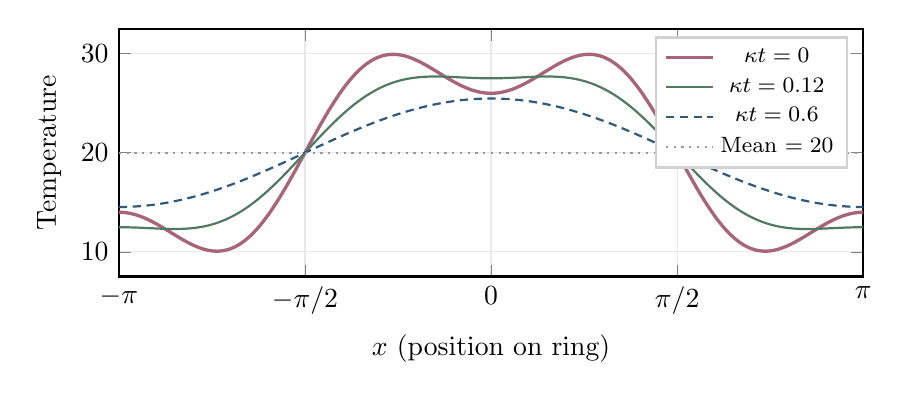
\begin{tikzpicture}
\begin{axis}[
 width=0.91\textwidth,height=0.39\textwidth,
 xmin=-3.14159,xmax=3.14159,ymin=7.5,ymax=32.5,
 xlabel={$x$ (position on ring)},ylabel={Temperature},
 xtick={-3.14159,-1.570796,0,1.570796,3.14159},
 xticklabels={$-\pi$,$-\pi/2$,$0$,$\pi/2$,$\pi$},
 grid=major,grid style={black!9},
 line width=0.85pt,
 legend style={at={(0.98,0.97)},anchor=north east,fill=white,
 draw=black!18,font=\footnotesize},
]
\addplot[color=pink,very thick,samples=250,domain=-3.14159:3.14159]
 {20+10*cos(deg(x))-4*cos(deg(3*x))};
\addlegendentry{$\kappa t=0$}
\addplot[color=green,thick,samples=250,domain=-3.14159:3.14159]
 {20+10*exp(-0.12)*cos(deg(x))-4*exp(-9*0.12)*cos(deg(3*x))};
\addlegendentry{$\kappa t=0.12$}
\addplot[color=deepblue,densely dashed,thick,samples=250,domain=-3.14159:3.14159]
 {20+10*exp(-0.6)*cos(deg(x))-4*exp(-9*0.6)*cos(deg(3*x))};
\addlegendentry{$\kappa t=0.6$}
\addplot[color=black!40,dotted,thick,samples=3,domain=-3.14159:3.14159]
 {20};
\addlegendentry{Mean $=20$}
\end{axis}
\end{tikzpicture}
\caption{Heat diffusion smooths out short-scale variations first, while the
mean temperature stays fixed. Curves are plotted at dimensionless times $\kappa t$.}
\label{fig:heat-plot}
\end{figure}

\subsection{Why the average temperature is conserved}
Define the spatial average $\mean{u}(t)$ by
\[
 \mean{u}(t)=\frac{1}{2\pi}\int_{-\pi}^{\pi}u(x,t)\,dx.
\]
For a smooth periodic solution, differentiate under the integral:
\begin{align*}
 \frac{d\mean{u}}{dt}
 &=\frac{\kappa}{2\pi}\int_{-\pi}^{\pi}u_{xx}(x,t)\,dx\\
 &=\frac{\kappa}{2\pi}\bigl[u_x(\pi,t)-u_x(-\pi,t)\bigr]=0.
\end{align*}
Hence the average temperature is always $\mean{u}(t)=c_0$.
This is also clear from \cref{eq:heat-solution}: the $n=0$ term has the factor
$\ee^{-\kappa\cdot0^2t}=1$.

All terms with $n\neq0$ decay to zero as $t\to\infty$, so
\begin{equation}\label{eq:equilibrium}
 \boxed{u(x,t)\longrightarrow c_0
 =\frac{1}{2\pi}\int_{-\pi}^{\pi}f(x)\,dx.}
\end{equation}
For an insulated ring, \emph{heat is redistributed rather than lost}. The
final temperature is uniform and equal to the initial average.

\subsection{A stronger statement: fluctuations lose energy}
For real-valued $u$, let $v(x,t)=u(x,t)-c_0$. Define the squared size of the
temperature fluctuations by
\[
 E(t)=\frac12\int_{-\pi}^{\pi}v(x,t)^2\,dx.
\]
Since $v_t=\kappa v_{xx}$, integration by parts gives
\begin{align}\label{eq:energy}
 E'(t)
 &=\int_{-\pi}^{\pi}v v_t\,dx
 =\kappa\int_{-\pi}^{\pi}v v_{xx}\,dx\notag\\
 &=\kappa[vv_x]_{-\pi}^{\pi}
 -\kappa\int_{-\pi}^{\pi}(v_x)^2\,dx
 =-\kappa\int_{-\pi}^{\pi}(u_x)^2\,dx\leq0.
\end{align}
The boundary term vanishes because the solution is periodic. Thus the spatial
variation, measured by $E(t)$, can only decrease. This also gives uniqueness:
if two solutions have the same initial condition, apply the identity to their
difference to see that the difference must stay zero.

\subsection{An initial square-wave temperature}
\begin{example}[Discontinuous initial data]
Even an idealized discontinuous initial temperature can be handled. If
\[
 f(x)=20+10\sgn(\sin x)
\]
away from its jump points, then \cref{eq:square} gives
\begin{equation}\label{eq:square-heat}
 u(x,t)=20+\frac{40}{\pi}\sum_{k=0}^{\infty}
 \frac{\ee^{-\kappa(2k+1)^2t}}{2k+1}
 \sin\bigl((2k+1)x\bigr),\qquad t>0.
\end{equation}
The higher odd harmonics disappear rapidly, so the once-discontinuous profile
becomes smooth for every positive time.
\end{example}

\section{Two deeper connections}
\subsection{Heat diffusion is a frequency filter}
The heat equation changes Fourier coefficients according to
\[
 \underbrace{\widehat{u}_n(t)}_{\text{output}}
 =\underbrace{\ee^{-\kappa n^2t}}_{\text{frequency response}}
 \underbrace{c_n}_{\text{input}}.
\]
Low frequencies ($|n|$ small) change slowly; high frequencies ($|n|$ large)
are suppressed quickly. In signal-processing language, diffusion acts like a
\emph{low-pass filter}. A mode's characteristic decay time is
\[
 \tau_n=\frac{1}{\kappa n^2}\quad(n\neq0).
\]

\subsection{Beyond a ring of circumference \texorpdfstring{$2\pi$}{2 pi}}
For a periodic interval of length $L$, the appropriate modes are
$\ee^{2\pi inx/L}$. The coefficient and heat-evolution formulas become
\begin{align*}
 c_n&=\frac1L\int_{-L/2}^{L/2}
 f(x)\ee^{-2\pi inx/L}\,dx,\\
 u(x,t)&=\sum_{n\in\ZZ}c_n
 \exp\!\left[-\kappa\left(\frac{2\pi n}{L}\right)^2t\right]
 \ee^{2\pi inx/L}.
\end{align*}
The general principle is even broader: if a linear spatial operator has a
useful eigenfunction basis, expanding in that basis can turn a PDE into many
independent ODEs. This is why closely related ideas appear in vibrating strings,
quantum mechanics, optics, and signal processing.


\section{Practice problems}
\begin{problem}[Check your understanding]
\leavevmode\par\smallskip
\begin{enumerate}
 \item Find every nonzero complex Fourier coefficient of
 $f(x)=3+2\cos(2x)-\sin(3x)$.
 \item Prove that if $f$ is real-valued, then $c_{-n}=\overline{c_n}$.
 \item Suppose $f(x)=12+5\cos(2x)+3\sin(5x)$ is the initial temperature
 on a circular rod. Write $u(x,t)$ and its limiting temperature.
 \item A temperature profile contains equal-amplitude modes of frequencies
 $2$ and $6$. How many times faster is the exponential decay rate of the
 frequency-$6$ mode?
 \item Explain why the Fourier series of the square wave equals $0$ at its
 jumps rather than $1$ or $-1$.
\end{enumerate}
\end{problem}

\subsection*{Answers and hints}
\begin{enumerate}
 \item $c_0=3$, $c_{2}=c_{-2}=1$, $c_3=i/2$, $c_{-3}=-i/2$.
 \item Conjugate the integral in \cref{eq:coefficients} and use
 $\overline{f(x)}=f(x)$.
 \item $u(x,t)=12+5\ee^{-4\kappa t}\cos(2x)
 +3\ee^{-25\kappa t}\sin(5x)$; the limiting temperature is $12$.
 \item The decay rates are proportional to $n^2$, so the ratio is
 $6^2/2^2=9$.
 \item By the pointwise convergence theorem, the sum at a jump equals the
 midpoint of the left and right limits, namely $(-1+1)/2=0$.
\end{enumerate}


\end{document}